\chapter{Initial Survey}

An enormous quantity of researches, which is sponsored by industry companies or
universities, was executed to find a better approach to stabilize \UAV by
using different sensors. Movement detection approaches, which are ultrasonic, sonar or
\RF based, show that it is necessary to have known reference points to get a
reliable result 
\citebib[p.2 Ultrasound indoor localization with reference points]
{EckDreGer09}\citebib[pp.4-5 Radio Model Localization]{BulHeiEst02}.
 The problem of this approach is that the environment has to be prepared before
 the UAV flight.
 This preparation is a drawback in point of flexibility in different operation
 places. Anyway, approaches with ultrasonic, \RF or sonar sensors show that the
 localization of \UAV needs a kind of global feedback to correct the \UAV 
 absolute position. One of the first motivations for a vision based sensor was
 presented by Ettlinger et al. 
 \citebib[pp.1-2 Visual-Based Localization and Control]{EttNecIfjWas04}.
 In this paper, the authors suggest, that vision is the only practical solution
 for obstacles of flight stability and showed an On-board
approach for a \GUAV by detecting the horizon with a forward looking camera and
estimating and control the flight attitude. Further vision based attitude control
approaches also were used for \HUAV with the difference of a down looking
camera for reference point free movement detection or an Off-Board camera which
tracks the global position of the \UAV.


\section{On- vs. Off-Board Camera and Image Processing}

The Off-Board camera approach was researched by Altug et al.
\citebib[p.76 Localization and Control with an Off-Board camera]{AltOstMah02},
 with the result of a less sensitive feature detection and position localization
 as the On-Board camera approach. Off-Board camera tracking is also shown in the
developments of extremely reliable and precise localization of a \UAV and it is
actually used in the development of aggressive autonomous flights of multiple
\MAV in the experiments of Mellinger et al. 
\citebib[Trajectory Generation and Control with Off-Board cameras]
{MelMicKum10} \citebib[pp.363-364]{GurStuAchDotHirRus07}. The advantage of
the Off-Board camera tracking system is that the image capturing and position
tracking is executed outside the \UAV and prevents complex On-Board calculations
for movement and position estimation. The drawbacks of this Off-Board Tracking
methods are that they need a previous prepared testbed for the flying
environment, which is build up with a motion tracking system 
\citebib[pp.1-2 The GRASP Testbed]{MicMelLinKum10}.

Problems, such as a limited power resource, a poor level of algorithm complexity
for image processing resulting from the limited calculating On-Board performance
and the endeavour to economise weight, lead to outsourcing the image processing
to a remote system which is not concerned to the On-Board problems. Langer et al.
\citebib[pp.5-7 Off-Board Image Processing]{LanSuePro08} uses an Off-Board image
processing to track a landing pad for autonomous landing. Thereby the images are
transmitted in this approach over Wifi communication to a base station, which
tracks the landing pad and sends back information of position control. Thereby it was
shown that the landing algorithm has to run at maximal 100Hz to work with
the transmitting delays of the images.\newpage
 This landing algorithm shows that it is possible to outsource successfully the
 image processing in consideration of the sample rate which the algorithm needs.
By regarding the drawback of the image transmission delay of the Off-Board image
processing, On-Board approaches were developed with the focus to the Real-Time
behaviour. Tippetts \citebib[pp.21-22 On-Board image processing with an FPGA]
{Tip08} realized an On-Board approach with a \FPGA which uses a complex feature
tracking algorithm but runs with 100MHz sampling rate. The characteristics
of the feature tracking with a \FPGA can result a fast movement tracking method,
but it is not an efficient method in the behaviour of power consumption because
the hardware is not optimized for the image processing tasks.

%01.11.2010 Stoped here
\begin{figure}[!htbp]
	\centering
		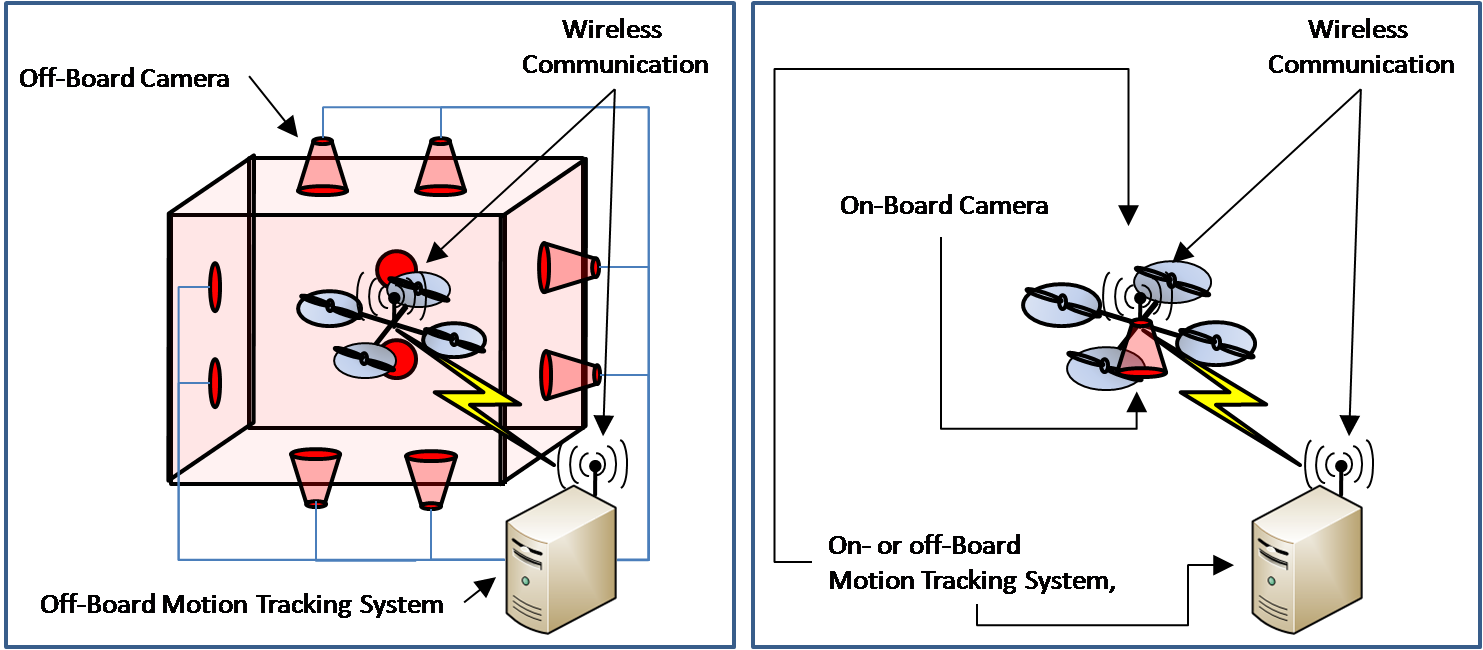
\includegraphics[width=0.85\textwidth]{graphic/Off-BoardvsOn-BoardCameras.png}
	\caption{On- and Off-Board camera and motion tracking system approach}
	\label{fig:Off-BoardvsOn-BoardCameras.png}
\end{figure}

\section{Hardware vs. Software-based image processing}

 In contrast to the drawbacks of \FPGA s, Langer et al.
\citebib[On-Board image processing with mice sensors]{LanSuePro09} and
 Beyeler et al. \citebib[pp.4-5]{BeyChrFlo09} showed an approach for detecting
 the spatial movement of a \UAV with optical mice sensors which have an optimized
 hardware for image processing and are lightweight.
 \newpage
 These sensors calculate the optical flow of the captured images and estimates
 the movement direction of the \UAV in hardware and
can provide a high sample rate. In contrast to the fast movement detection,
a disadvantage, is that these sensors have limitations related to the operating
environments. These limitations are the concrete light and distance range which
is required from the manufacturer 
\citebib[pp.7-15 Limitations of the operating environment] 
{ST05_1}. The most of the experiments with a stabilisation approach with mice
sensors uses optical lens to reach a higher degree of operating distance, but the
effort in most of the cases is not satisfactorily to the results as Langer et.
al have shown
 \citebib [p.6 Performance of the optical flow based position controller] 
 {LanSuePro09}. Software based image processing approaches have a more flexible
 extension and change behaviour, but they work not as fast as hardware based
 approaches. Further advantages of software based image processing are, that the
most of the commercial and open source computer vision \API also provide
implemented estimators and filters to correct the captured input and to decrease
noise of the images. Stowers et al. realized a heading estimation for a
quadrocopter with an onboard \SBC which runs the open source computer vision
toolkit OpenCV\citebib[The OpenCV Reference]{OpenCV2_0}. This software based
image processing approach shows strengths in the modularity of the image processing architecture and in the interchangeability
of the vision system \citebib [pp.1-6 Software Based Vision Processing]
{StoBaiHayMil09}\citebib[Software Structure and Porability]{GarKae08}.

\newpage
\section{Vision based movement detection approaches}

Sequential captured images contain a huge amount of information about the
absolute and relative movement of objects in every direction. So several vision
based movement detection approaches were researched in the topic of \UAV
stabili- sation with different requirements to the information which extracted
from the vision process. A simple approach for a relative vision based control of
a \UAV was implemented by Boabdallah \citebib[pp.110-114 Position Sensor]{Bou07}
by using a down looking camera and the Canny edge detector \citebib{Can86} and
the Douglas Peuker Algorithm for curve equalisation \citebib{DouPeu73}. The drawback of this approach is that the field of vision must contain forms with edges which mean that the approach cannot result a satisfactory result if no
edges are detected. A further approach for detecting relative movements and to
build up a map for autonomous navigation, is visual \SLAM. This approach tracks
features in the field of vision and reconstructs a relation to tracked features
of previous images. The realization of \SLAM \citebib{WilKleRei07} in a \UAV
was executed in the work of Bloesch et al. \citebib{BloWeiScaSie10} under
consideration of real-time characteristics. The behaviour of the algorithm shows
that the localization of the tracked features and the simultaneous mapping has a
big impact at the time delay of the calculation. So the experiments and the
control algorithms were researched and designed for 7.5Hz sample rate. Another
popular tracking method for movement detection is given with the Optical Flow,
which can be described as movement observation of tracked objects or pixels in a
sequence of images. Algorithms to calculate the Optical Flow were introduced by
Horn and Schunk \citebib{HorSch80}, Lukas and Kanade \citebib{LucKan81}.
\newpage A few years after introducing the Lucas-Kanade-Algorithm, Lucas
described the theoretical approach of visual navigation by using the Optical Flow. Thereby he
described the possibility to detect movements and to calculate correspondence
velocities. These velocities can be combined to a vector field which can describe
movements in every direction 
\citebib[pp.40-45 Optical Navigation Theory]{Luc84}.


\begin{figure}[!htbp]
	\centering
		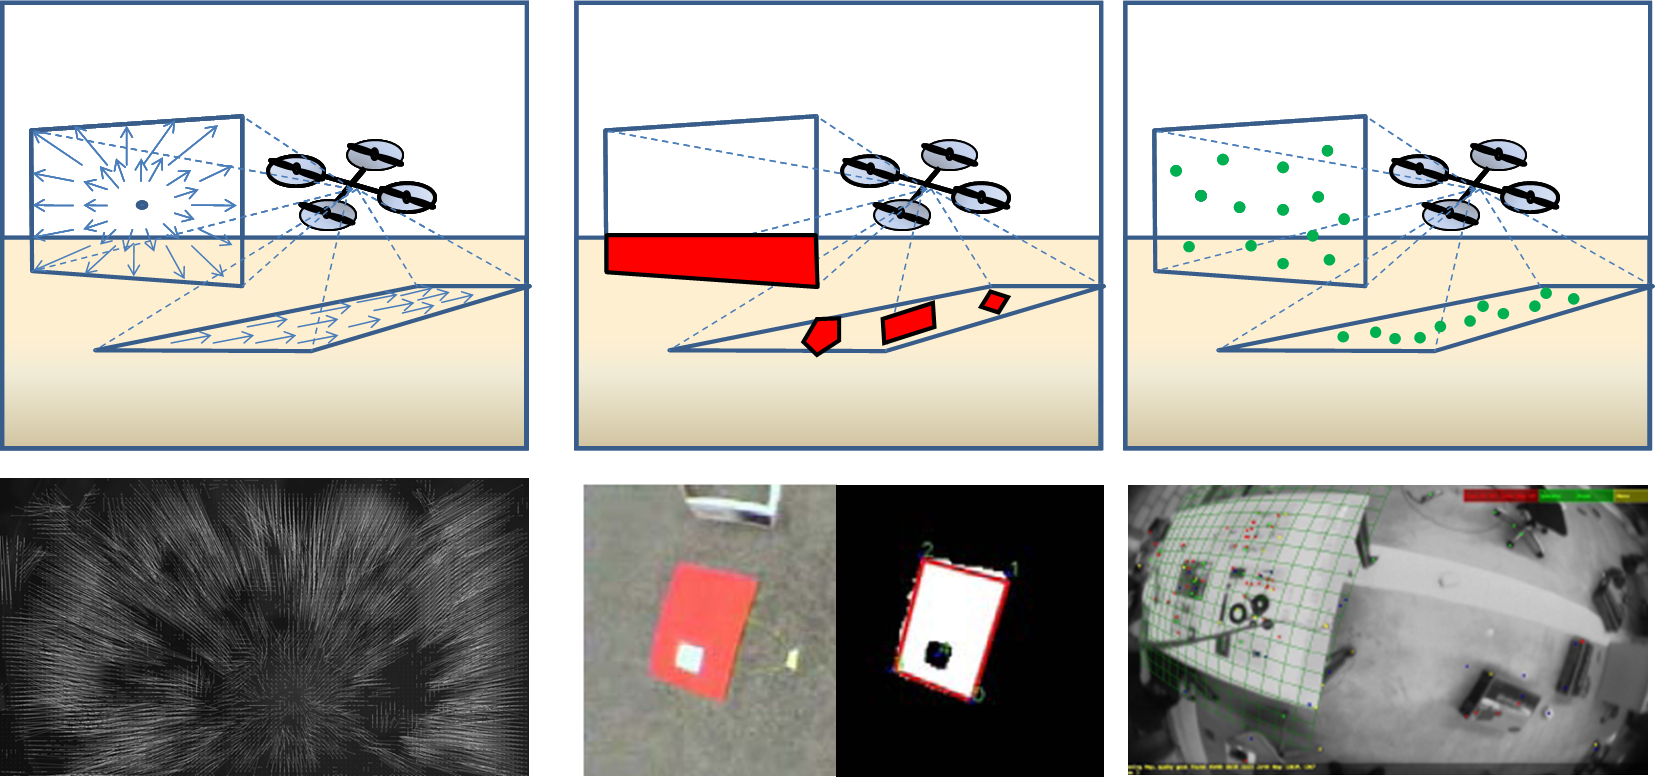
\includegraphics[width=0.75\textwidth]{graphic/VisualApproaches.png}
	\caption{Samples for UAV stabilisation with Optical Flow, Edge detection and SLAM}
	\label{fig:VisualApproaches.png}
\end{figure}

\newpage
\section{Control Approaches}

The closed loop feedback architecture is an approved method for controlling
systems and nearly used in the most of the systems controls in industry and
society. So the most of the researches in the \UAV stabilisation topic were
and still are executed with closed loop control architectures which are built up as
\MIMO systems. The differences between the researched approaches are the
amount of the inputs and outputs of the physical process, the type of controller,
the used measurements and the sampling rate. Thereby the type and behaviour of
the controller is close related to the measurements and the physical process
\citebib[p.3]{DorBis01}.
 The classical control approach using \PID controler was
researched in several \HUAV projects \citebib[pp.24-31]{Sik08}
\citebib[pp.43-68] {Bou07}. These researches show that the \PID control is not
robust enough to handle with measurement errors and to control multiple \DOF s. So the most of
the released control approaches with \PID technique extends the control architecture
with estimators and filters to get more precise measurements. Another
approach for control improvement was introduced by Luenberger \citebib{Lue71} and
describes a closed loop control approach, called state-observer, which simulates
the process in real time parallel to the true process by using the input and
output vector of the closed loop system and corrects the control strategy.
Bloesch et al. \citebib[p.5] {BloWeiScaSie10} have shown in their research,
that the problematic of sensors with non-negligible time delay can be solved to an
adequate result by using a state-observer.\newpage The reason for that is that
the state-observer allows configurate and to control the stability behaviour of the
closed loop feedback architecture. If a process can be observed or furthermore
controlled, is related to the states in which it can be and furthermore to
 the measurements of the \DOF 
 \citebib [pp.632-636 Controllability and Observability]{DorBis01}. In this
 project it has to be determined how correction values which are provided
 from the optical sensor with a slower sampling rate, can include into the
 control algorithm of the aircraft.


\begin{figure}[!htbp]
	\centering
		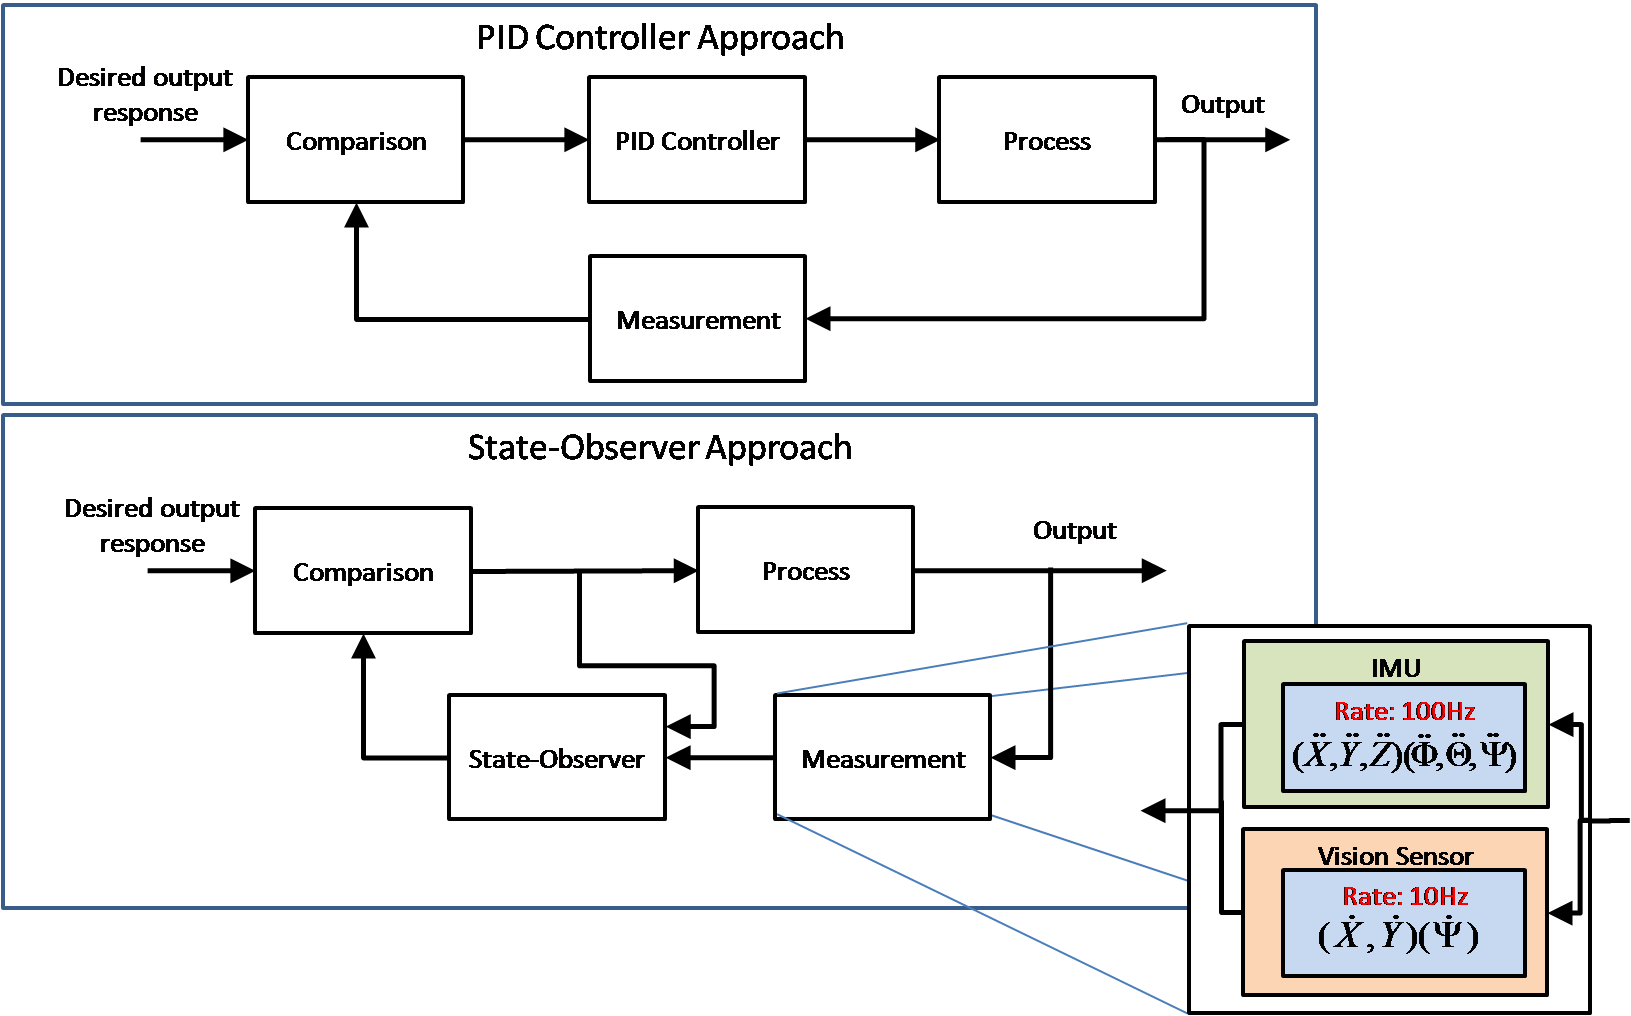
\includegraphics[width=0.75\textwidth]{graphic/ClosedLoopControlSyst.png}
\caption
{PID-Controler and State-Observer in closed loop System with variable sample sensor rates}
	\label{fig:ClosedLoopControlSyst.png}
\end{figure}

\newpage
\section{Proposed Approach}

This chapter shows several approaches for movement detection and stabilisation of
\UAV. The found methods were critically analyzed and assessed with the result
to investigate the following techniques which are shown in figure \ref{fig:ProposedApproach.png}.
 The proposed solution to eliminate the stabilisation problems of the
 quarocopter has to be vision-based for achieving the goal of flexibility and independence of
operational environment. Related to the off-board image processing, the problem
of the processing delay, could be solved with a state-observer. Furthermore the
optical movement detection should work without reference points.
 So the optical flow method has to be researched by using a
software-based detection approach for more flexibility and replaceability.
Because the approach of the flight control is teleoperated and the flight
stabilisation does not have to provide aggressive flight maneuvers, it is simpler
to realize the camera view on-board. This proposed solution has to be simulated
 to check the feasibility and to determine the limitations.


\begin{figure}[!htbp]
	\centering
		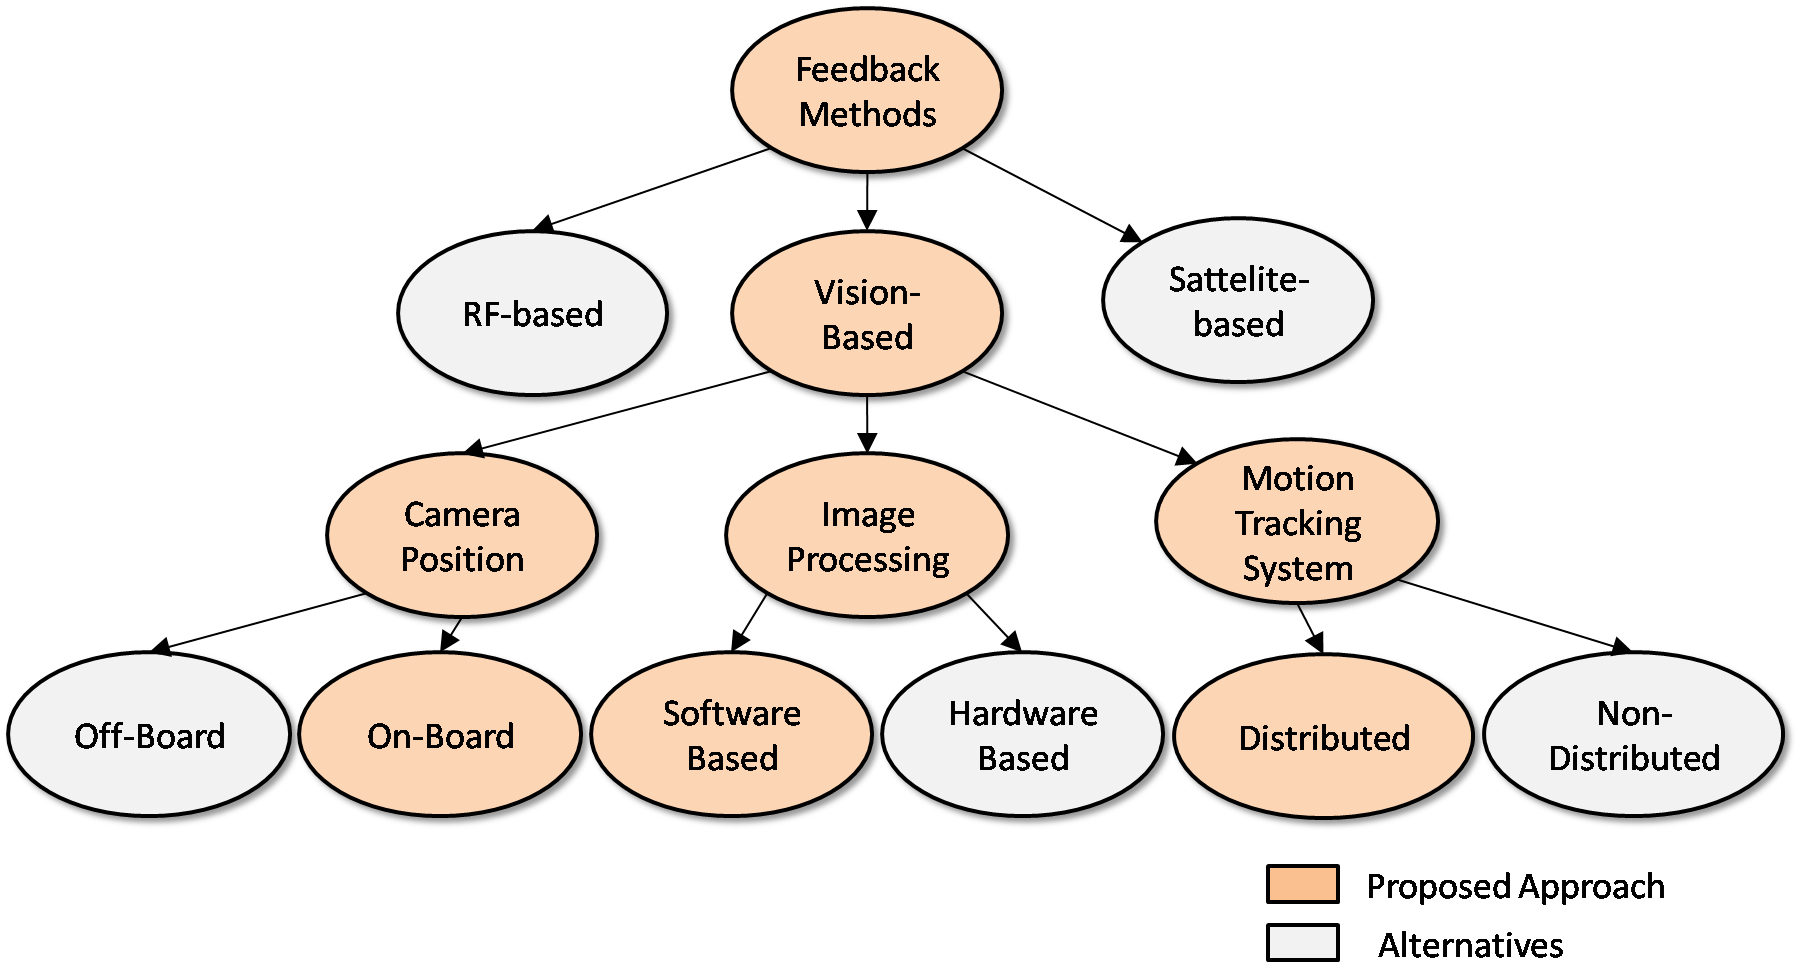
\includegraphics[width=0.75\textwidth]{graphic/ProposedApproach.png}
\caption
{Proposed Approach}
	\label{fig:ProposedApproach.png}
\end{figure}
